\documentclass[11pt,a4paper,spanish,openany,twoside]{report}
\usepackage{csquotes}
\usepackage[spanish,es-tabla]{babel}
%allow for áéíóú
\usepackage[utf8]{inputenc}
%set page geometry for PRINTED version (more margin on the inner side towards the book's spine)
%\usepackage[top=2.25cm, bottom=2.25cm, outer=2cm, inner=3cm, heightrounded, marginparwidth=2.5cm, marginparsep=0.3cm]{geometry}
%set page geometry for PDF version
\usepackage[top=2.25cm, bottom=2.25cm, outer=2.5cm, inner=2.5cm, heightrounded, marginparwidth=2.5cm, marginparsep=0.3cm]{geometry}


%load images
\usepackage{graphicx}
\graphicspath{{Images/}}


%bibliography: add .bib file in Others/library.bib
%set bibliography style according to faculty specifications
\usepackage[%
	backend=bibtex       % biber or bibtex
	%,style=authoryear   % Alphabeticalsch
	,style=numeric-comp  % numerical-compressed
	,sorting=nty         % no sorting: none %nty (name title year)
	,sortcites=true      % some other example options ...
	,block=none
	,indexing=false
	,citereset=none
	,isbn=false
	,url=true
	,doi=false           % prints doi
	,natbib=true         % if you need natbib functions
]{biblatex}
\addbibresource{Others/library.bib}  
\setcounter{biburllcpenalty}{7000}
\setcounter{biburlucpenalty}{8000}
\usepackage{multicol}
\renewcommand*{\bibfont}{\scriptsize} %\tiny


%in-document links (LOAD LAST, math overwrites the reference system)
\usepackage[hidelinks]{hyperref}
\usepackage[capitalise]{cleveref}
\crefname{table}{tabla}{tablas}


%for adding dummy text
\usepackage[math]{blindtext}

\usepackage{titlesec}

\usepackage{parskip} 


%BEGIN THE DOCUMENT ITSELF
\begin{document}
	%Do not number pages until we are ready
	\pagenumbering{gobble} 
	
	%Place TOP COVER 
	% \begin{titlepage}
	%make sure this page is centered
	\newgeometry{top=2.25cm, bottom=2.25cm, outer=2.5cm, inner=2.5cm, heightrounded, marginparwidth=2.5cm, marginparsep=0.3cm}
	\thispagestyle{empty}

	\begin{center}

		\vspace{1cm}

		\vspace{0.65cm}
		\rule{2in}{0.5pt}\\
		\vspace{0.85cm}

		{\Large Multisource RF SIGINT}\\

		\vspace{0.65cm}
		\rule{2in}{0.5pt}\\
		\vspace{0.85cm}

		{\Large Inteligencia de Señales desde diversas fuentes de radiofrecuencia}\\

		\vspace{0.65cm}
		\rule{2in}{0.5pt}\\
		

		\vfill
		
\includegraphics[height=2.5in]{escudo_ucm.pdf}
		\vfill

		

		\textbf{TRABAJO DE FIN DE GRADO}\\
		\vspace{0.7cm}
		\textbf{Marcos Alonso Campillo}

		\vspace{1cm}

		Directores:\\
		\textbf{José Luis Vázquez Poletti}\\
		\textbf{Juan Carlos Fabero Jiménez}

		\vspace{1.8cm}
		Facultad de plantillas de \LaTeX\\
		Universidad Complutense de Madrid
		\vspace{0.5cm}
	   
		1 de Enero del 2024

		\vspace{0.2cm}

	\end{center}
\end{titlepage}
	\clearpage

	%Place authorship declaration
	%and financial support on its back 
	% {
	\newcommand{\checkbox}{{\fboxsep=-.15pt\fbox{\rule{0pt}{1.5ex}\rule{1.5ex}{0pt}}}}
	
	\setlength{\parskip}{14pt}

	\noindent
\includegraphics[width=7cm]{logo_alargado_ucm.jpg}
	\vspace{0.5cm}
	\begin{center}
		\textbf{AUTORIZACIÓN PARA LA DIFUSIÓN DEL TRABAJO FIN DE GRADO Y SU DEPÓSITO EN EL REPOSITORIO INSTITUCIONAL E-PRINTS COMPLUTENSE}
	\end{center}
	\vspace{0.5cm}

	\noindent Los abajo firmantes, alumno/s y tutor/es del Trabajo Fin de Grado (TFG) en el Grado en 
	NOMBRE DEL GRADO REALIZADO de la Facultad de NOMBRE DE LA FACULTAD, autorizan a la Universidad Complutense de Madrid (UCM) 
	a difundir y utilizar con fines académicos, no comerciales y mencionando expresamente 
	a su autor el Trabajo Fin de Grado (TFG) cuyos datos se detallan a continuación. 
	Así mismo autorizan a la Universidad Complutense de Madrid a que sea depositado en acceso abierto
	en el repositorio institucional con el objeto de incrementar la difusión, 
	uso e impacto del TFG en Internet y garantizar su preservación y acceso a largo plazo. 

	\noindent Periodo de embargo (opcional): 

	\quad \checkbox\ 6 meses 
	
	\quad \checkbox\ 12 meses 

	\vspace{0.5cm}

	\noindent \textbf{Título del TFG: Inteligencia de Señales desde diversas fuentes de radiofrecuencia}

	\noindent \textbf{Curso académico: } 2023/2024    
	
	\noindent \textbf{Nombre del Alumno/s: Marcos Alonso Campillo}
	
	\noindent \textbf{Tutor/es del TFG y departamento al que pertenece:  José Luis Vázquez Poletti, Juan Carlos Fabero Jiménez}

	\vspace{1cm}

	\begin{center}
		En Madrid, a \today

		\vspace{1cm}

		Firma del alumno \hfill Firma del director/es
	\end{center}
}
	\clearpage
	
	%Place dedication
	% {
    \raggedleft
    \emph{Dedicado a ranita.}


    \ \\
    \ \\

    \emph{To whomever who uses this template.}
    
}
	\clearpage

	%Start numbering pages with roman numbers
	\pagenumbering{roman}
	% \chapter*{Agradecimientos}
	\addcontentsline{toc}{chapter}{Agradecimientos} 

		\Blindtext[8]
	% \chapter*{Abstract}
	\addcontentsline{toc}{chapter}{Abstract}

	An innovative solution is presented in the field of Open Source Intelligence (OSINT), focusing on the Automatic Packet Reporting System (APRS). The developed tool consists of a system designed to collect, process, and analyze real-time data from APRS packet transmitters.

	The utility of the APRS reporting system extends to diverse contexts such as weather station monitoring, emergency resource management, and vehicle tracking. However, the complexity of data generated by APRS transmitters and the lack of specialized tools for analysis hinder the extraction of relevant information and the identification of significant patterns.

	The proposed solution addresses this need by providing a platform for the automated collection of APRS data, processing it to extract relevant information, and analyzing it to identify patterns. The goal is to assist users in extracting useful information from the collected data.
    
    \textbf{Keywords}: OSINT, APRS, Analysis, Data, Proccessing.



\chapter*{Resumen}
	\addcontentsline{toc}{chapter}{Resumen}

	Se presenta una solución innovadora en el campo del Open Source Intelligence (OSINT), centrada en el sistema APRS de reporte automático de paquetes. La herramienta que se ha desarrollado consiste en un sistema diseñado para recopilar, procesar y analizar datos en tiempo real provenientes de emisores de paquetes APRS.

	La utilidad del sistema de reporte APRS se extiende a contextos tan diversos como pueden ser el monitoreo de estaciones meteorológicas hasta la gestión de recursos en casos de emergencias y el seguimiento de vehículos. Sin embargo, la complejidad de los datos generados por los emisores APRS y la falta de herramientas especializadas para su análisis dificultan la extracción de información relevante y la identificación de patrones significativos.

	La solución que se propone aborda esta necesidad proporcionando una plataforma para la recopilación automatizada de los datos APRS, procesándolos para extraer información relevante y analizándolos para identificar patrones con el objetivo de ayudar a los usuarios a extraer información útil de los datos extraidos.
    
    \textbf{Palabras clave}: OSINT, APRS, Análisis, Datos, Procesamiento.
	\clearpage


	%Table of contents, list of figures, list of tables
	\tableofcontents 
	\newpage
	\phantomsection\addcontentsline{toc}{chapter}{\listfigurename} %add LOF to index
	\listoffigures
	\newpage
	\phantomsection\addcontentsline{toc}{chapter}{\listtablename} %add LOT to index
	\listoftables
	\clearpage

    
	%capítulos
	\pagenumbering{arabic} 
	\titleformat{\chapter}[display]
{\normalfont\huge\bfseries}{Capítulo \thechapter}{0.5em}{\huge}
\titlespacing*{\chapter}{0pt}{-1.25cm}{25pt}
\chapter{Introducción}
\section{¿Qué es APRS?}

APRS o Sistema Automático de Reporte de Paquetes (APRS, por sus siglas en inglés: Automatic Packet Reporting System) es un sistema de comunicaciones digitales en tiempo real que permite el intercambio de información entre estaciones de radioaficionados.

De manera general, APRS se utiliza para el rastreo de vehículos, la transmisión de mensajes de texto, la diseminación de información meteorológica y la comunicación en situaciones de emergencia aunque debido a la flexibilidad del protocolo puede ser usado en cualquier otra situación.

\begin{figure}[h!]
	\centering
	
\includegraphics[width=0.2\textwidth]{./Chapter_1/APRS_logo.png}
	\caption{Logo de APRS.}
	\label{fig:aprs-logo}
\end{figure}

\section{Características Principales de APRS}

APRS posee varias características que lo hacen útil y versátil en el ámbito de la comunicación de radioaficionados, entre las cuales se encuentran las siguientes:
\begin{itemize}
	\item \textbf{Frecuencia de Operación:} APRS opera en la banda de VHF, específicamente en la frecuencia de 144.80 MHz en Europa, aunque en otras regiones del mundo se utilizan frecuencias diferentes tal como se muestra en la figura \Cref{fig:freq-map}.
	\item \textbf{Modo de Transmisión:} APRS utiliza como modo de transmisión paquetes individuales que han de seguir un formato establecido, esto facilita enormemente la adopción e integración de esta tecnología.
	\item \textbf{Actualización de Datos en APRS:} En el sistema APRS, un paquete de información se transmite múltiples veces, disminuyendo gradualmente la frecuencia de envio de estas transmisiones a medida que el tiempo avanza. Este método tiene como objetivo maximizar la tasa de recepción de los paquetes.
\end{itemize}

\begin{figure}
	\centering
	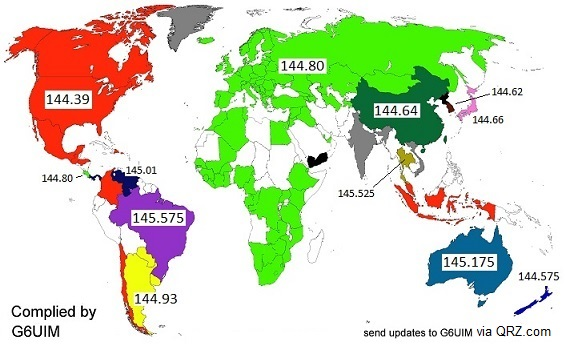
\includegraphics[width=0.5\textwidth]{./Chapter_1/mapa_frecuencias_aprs.jpg}
	\caption{Mapa de frecuencias APRS en el mundo.}
	\label{fig:freq-map}
\end{figure}


\section{Usos Principales de APRS}

\begin{itemize}
	\item \textbf{Reportes GPS:} APRS permite a los usuarios enviar su ubicación geográfica en forma de coordenadas, obtenida a través de sistemas GPS, lo que facilita el seguimiento de vehículos o personas en tiempo real.

	\item \textbf{Datos Meteorológicos:} Las estaciones meteorológicas suelen utilizar mensajes APRS para reportar diferentes datos como temperatura, humedad o presión barométrica, incluyendo información actualizada y útil para diversas aplicaciones.

	\item \textbf{Integración con Internet:} Mediante el sistema APRS-IS, los mensajes APRS son accesibles por internet a través de distintos nodos, ampliando el alcance y la extensión de este sistema.

	\item \textbf{Uso en Emergencias:} En situaciones de emergencia, APRS es una herramienta vital para la comunicación de broadcast y el seguimiento de recursos y personal.
\end{itemize}

\section{Historia y Desarrollo de APRS}

El sistema APRS nació en la decada de los 80 de la mano de Bob Bruninga, un ingeniero que trabajaba como en la Academia Naval de los Estados Unidos. Bruninga creó la primera implementación de APRS en un ordenador Apple II en 1982 con el objetivo de mapear informes de posición de la Marina en alta frecuencia.\footnote{\url{http://www.aprs.org/APRS-docs/ARTICLES.TXT}}

El primer uso real del APRS fue en 1984, cuando Bruninga desarrolló una versión más avanzada en un VIC-20 para reportar la posición y el estado de los caballos de una carrera de resistencia.

Durante los siguientes años, Bruninga continuó perfeccionando el sistema, al que posteriormente bautizó como Sistema de Tráfico de Emergencia Sin Conexión (CETS, por sus siglas en inglés).

Tras una serie de ejercicios de la Agencia Federal de gestión de Emergencias (FEMA) usando CETS, el sistema fue trasladado al IGM pC. Durante la década de los 90, CETS (ya conocido como el Sistema de Reporte Automático de Posición) continuó evolucionando.

A medida que la tecnología GPS se volvía más ampliamente disponible, el término "Posición" fue reemplazado por "Paquete" para encapsular mejor las capacidades más genéricas del sistema y enfatizar sus usos más allá del mero reporte de posición.
 
\begin{figure}[h!]
	\centering
	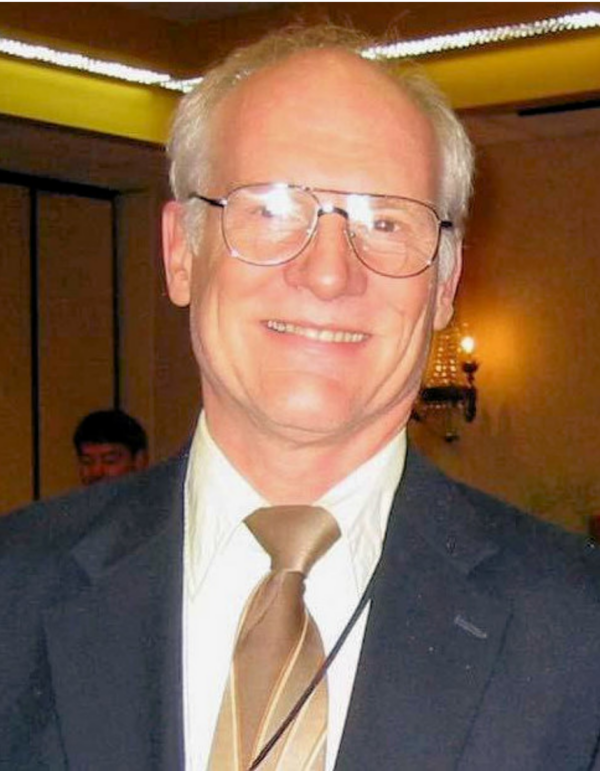
\includegraphics[width=0.25\textwidth]{./Chapter_1/bob_bruninga.png}
	\caption{Bob Bruninga.}
	\label{fig:bob-bruninga}
\end{figure}
	\titleformat{\chapter}[display]
{\normalfont\huge\bfseries}{Capítulo \thechapter}{0.5em}{\huge}
\titlespacing*{\chapter}{0pt}{-1.25cm}{25pt}
\chapter{Contexto del problema y estado del arte}

\section{Contexto del problema}

El \textit{Automatic Packet Reporting System} (APRS) como sistema de comunicación digital se basa en la gran comunidad de radioaficionados e incluso tiene aplicaciones industriales como la transmisión de información en tiempo real de vehículos logísticos o estaciones de meteorología. A pesar de su versatilidad y flexibilidad, el APRS presenta algunas barreras de entrada para usuarios que no pertenecen a la comunidad radioaficionada o tienen sólidos conocimientos de este ámbito. En este capítulo, se analizarán estas barreras y se discutirán los requisitos necesarios.

\subsection{Barreras de entrada}

El APRS requiere conocimientos básicos sobre radiocomunicación y la obtención de una licencia de radioaficionado en caso de querer emitir. La obtención de la licencia a pesar de no implicar un desembolso económico importante, si que requiere un estudio y comprensión de los sistemas y legislación pertinente.

Adicionalmente, el APRS utiliza una estructura de mensaje específico y un conjunto de protocolos que pueden ser difíciles de entender para usuarios no familiarizados con este tipo de tecnología. La falta de documentación y antigüedad de esta hacen que desarrollar soluciones para este sistema sea complicado.

\subsection{Hardware}

Para utilizar APRS, se necesita hardware especializado que incluya un transceptor de radio, un \textit{Terminal Node Controller} (TNC) y un dispositivo GPS (opcionalmente), existen otras opciones más baratas como los dispositivos \textit{software defined radio} o RTL-SDR \Cref{fig:rtl-sdr} que se conectan directamente a un ordenador. Los TNC son dispositivos que convierten las señales digitales emitidas por un ordenador en señales de radio y viceversa. El dispositivo GPS proporciona información de ubicación que se puede transmitir junto con otros datos en el cuerpo del mensaje.

El precio del hardware APRS puede variar dependiendo de la calidad y las características del equipo. Sin embargo, a pesar de no contar con precios prohibitibamente altos, la inversión que supone conlleva el hecho de que solamente los usuarios con un interés previo en la radioafición o la tecnología en general estén dispuestos a adquirirlo.

\begin{figure}
    \centering
    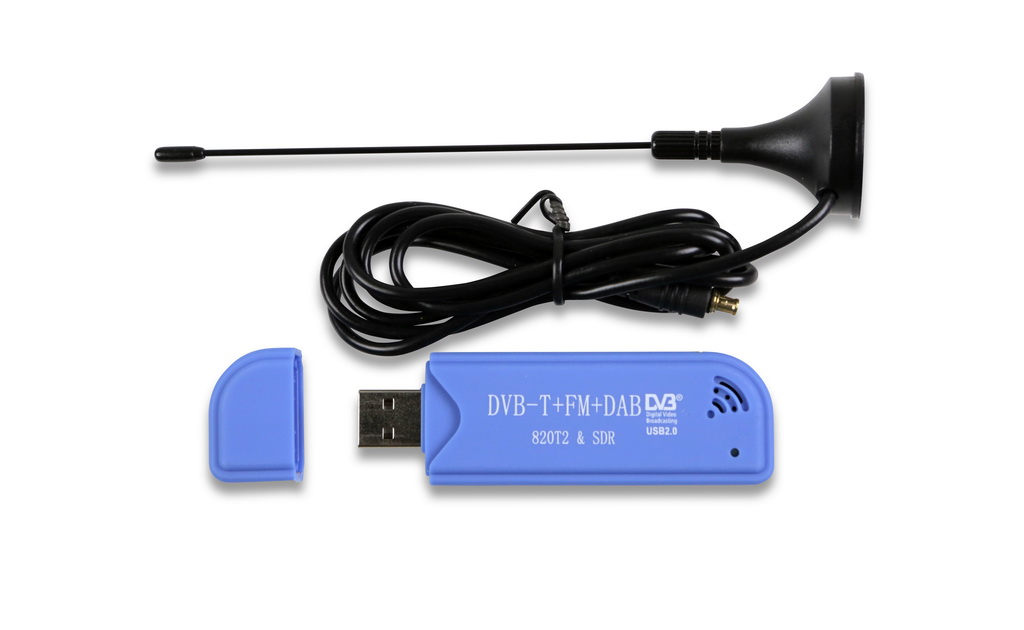
\includegraphics[width=0.5\textwidth]{./Chapter_2/rtl_sdr.jpg}
    \caption{Ejemplo de un RTL-SDR de tipo usb.}
    \label{fig:rtl-sdr}
\end{figure}


\subsection{OSINT y APRS}

El APRS sirve como una herramienta de comunicación para los radioaficionados y de reporte de telemetría para las industrias. Pero se puede convertir en una valiosa fuente de información para la obtención de inteligencia (OSINT). Esto se debe a su capacidad para proporcionar una gran cantidad de datos en tiempo real sobre ubicación y estado de los activos así como una amplia gama de información adicional.

En el ámbito del OSINT, el APRS ofrece una serie de aplicaciones prácticas. Por ejemplo, los datos APRS son actualmente utilizados para el rastreo de vehículos en tiempo real, lo que resulta muy útil para empresas de logística y transporte. Además, la red APRS se utiliza para monitorear la actividad de estaciones meteorológicas, proporcionando datos en tiempo real sobre condiciones climáticas locales. También se utiliza en situaciones de emergencia, como pueden ser desastres naturales o incidentes críticos, el APRS desempeña un papel crucial al permitir la transmisión rápida de información sobre ubicaciones de refugios, recursos disponibles y necesidades de ayuda, ya que no depende necesariamente de infraestructura de una entidad como si lo hace la red telefónica.

Aunque el APRS tiene un gran potencial para aplicaciones en el ámbito del OSINT, su uso en esta área es prácticamente inexistente. Este hecho puede explicarse en parte por las barreras de entrada mencionadas anteriormente, que incluyen la necesidad de poseer conocimientos especializados en radiocomunicación, obtener licencias de radioaficionado y adquirir hardware especializado.

\section{Estado del Arte}

Existen varios sitios web que ofrecen servicios relacionados con APRS, entre los cuales destacan \textbf{aprs.fi} y \textbf{aprs.to} probablemente las dos webs más grandes.

\subsection{aprs.fi}

aprs.fi es una de las webs más utilizadas para visualizar datos APRS en tiempo real y acceder a un histórico extenso de información. Sin embargo, su interfaz puede considerarse un tanto desactualizada (ver \Cref{fig:aprs-fi}), lo que puede dificultar la navegación y la búsqueda de información específica. Aunque ofrece una gran cantidad de datos y un histórico significativo, la plataforma carece de capacidades avanzadas de filtrado de estaciones y mensajes. Además, para acceder a funciones más complejas y realizar extracciones de datos, es necesario crear una cuenta.

\begin{figure}[h]
    \centering
    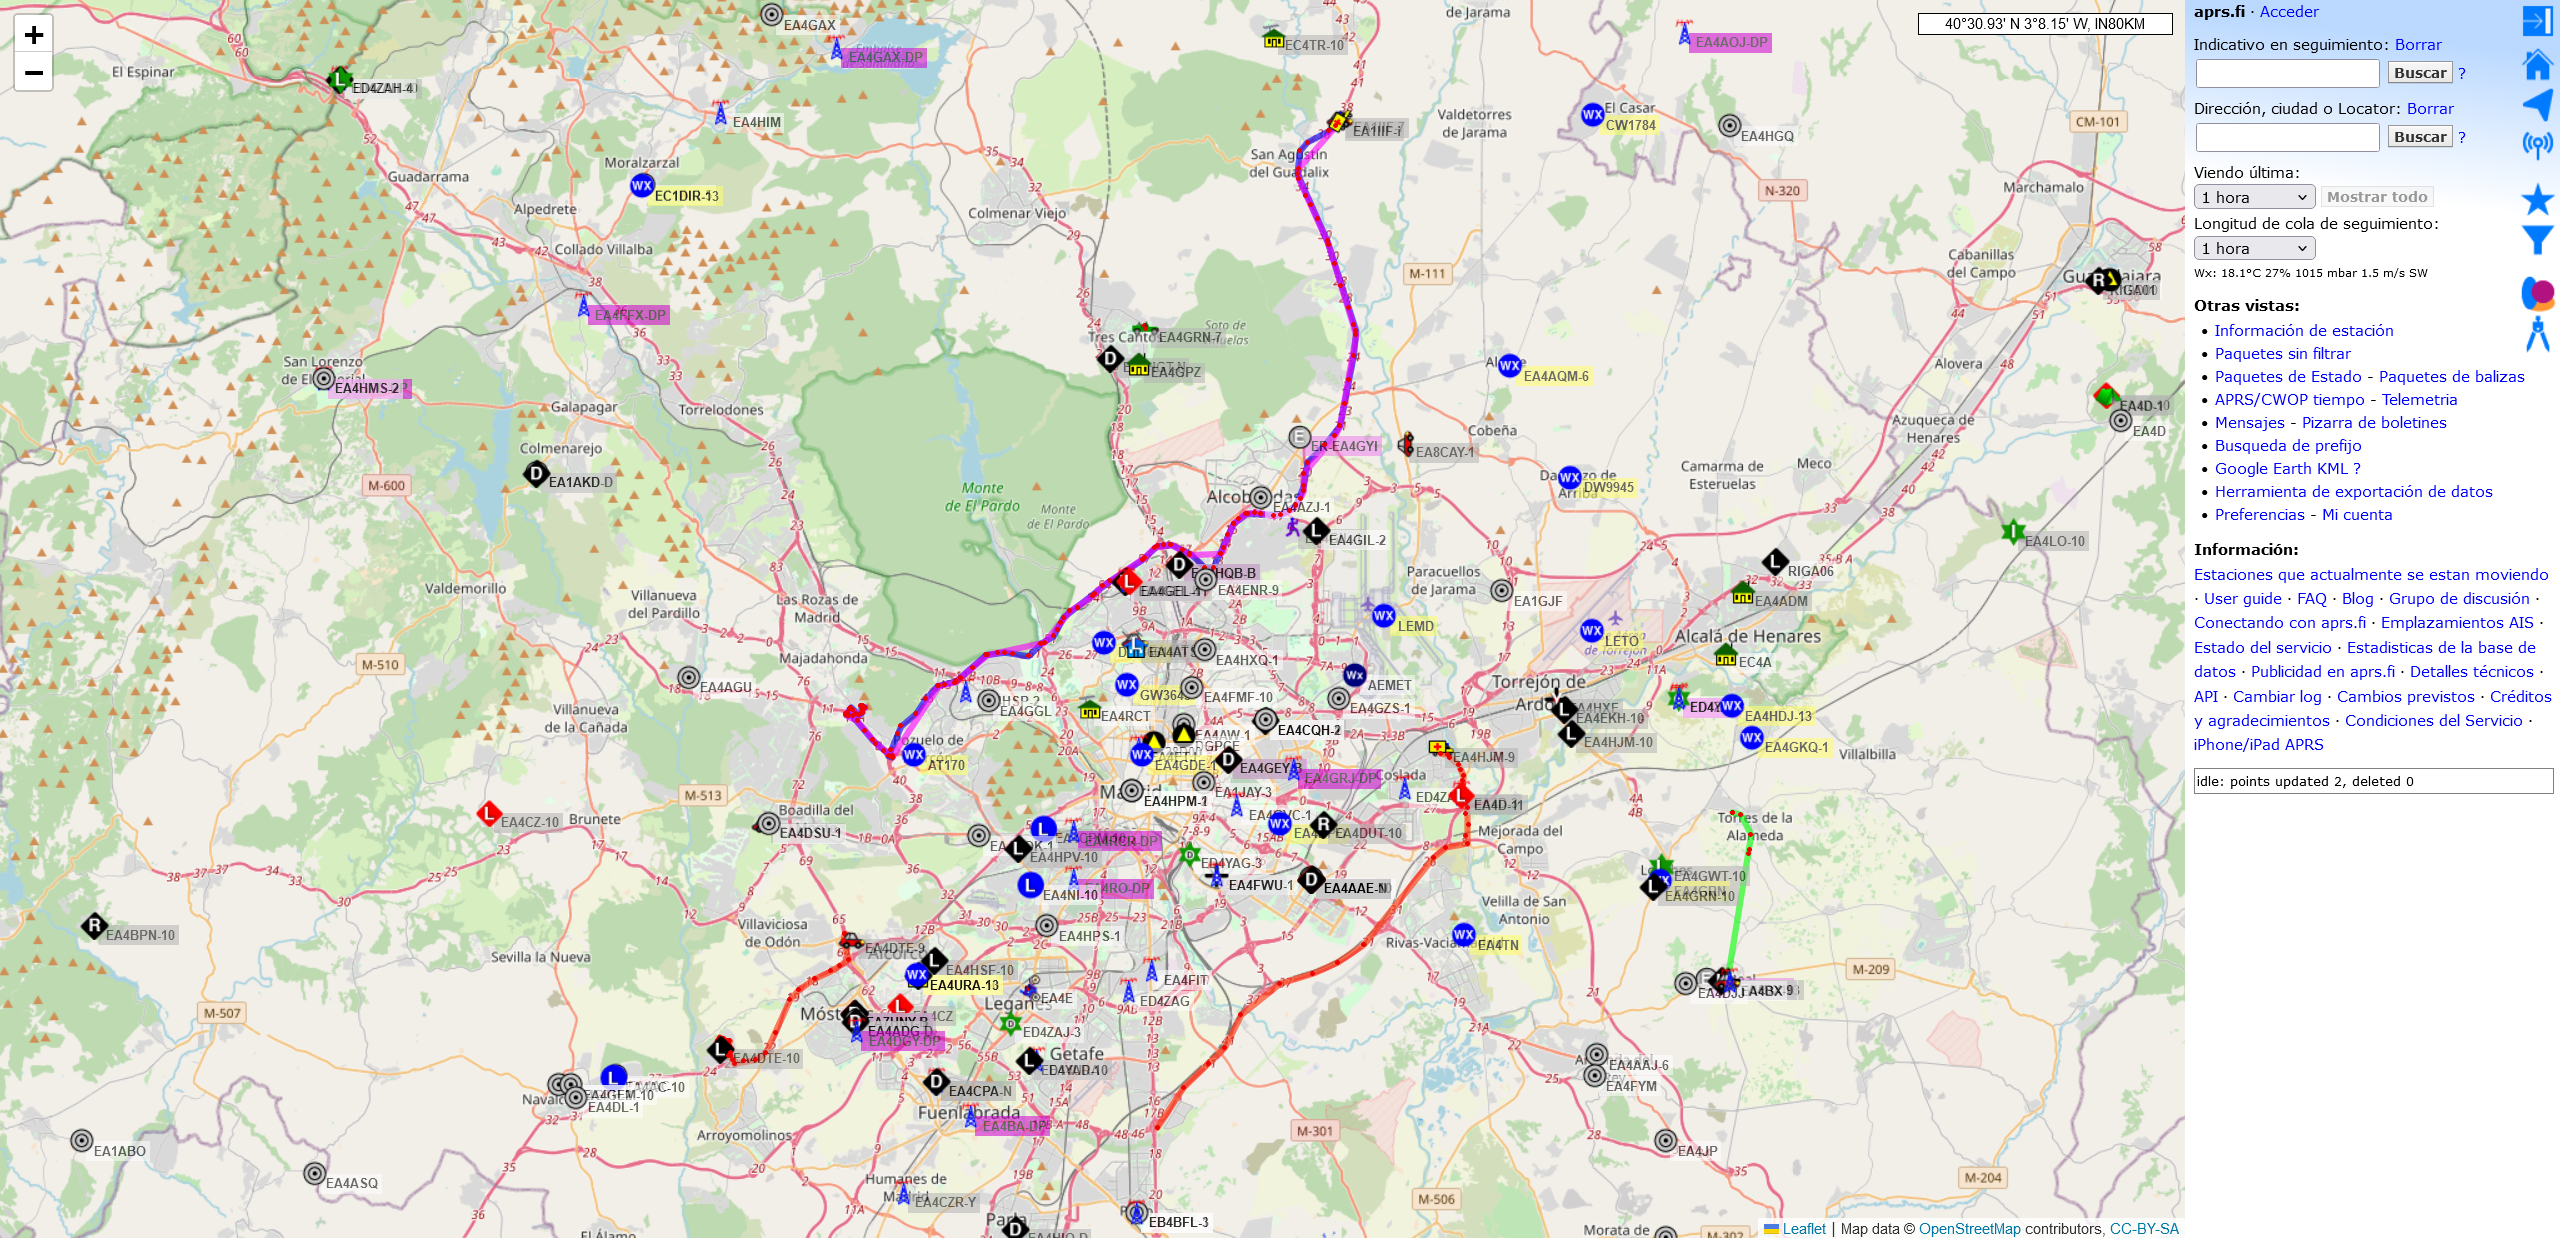
\includegraphics[width=0.7\textwidth]{./Chapter_2/aprs-fi.png}
    \caption{Interfaz de aprs.fi}
    \label{fig:aprs-fi}
\end{figure}

\subsection{aprs.to}

Por otro lado, aprs.to ofrece una interfaz más moderna y cuidada (ver \Cref{fig:aprs-to}), lo que facilita la navegación y la búsqueda de información. Además, permite realizar búsquedas básicas y aplicar filtros para refinar los resultados. Sin embargo, al igual que aprs.fi, también requiere que los usuarios se creen una cuenta para acceder a ciertas funcionalidades avanzadas.

\begin{figure}[h]
    \centering
    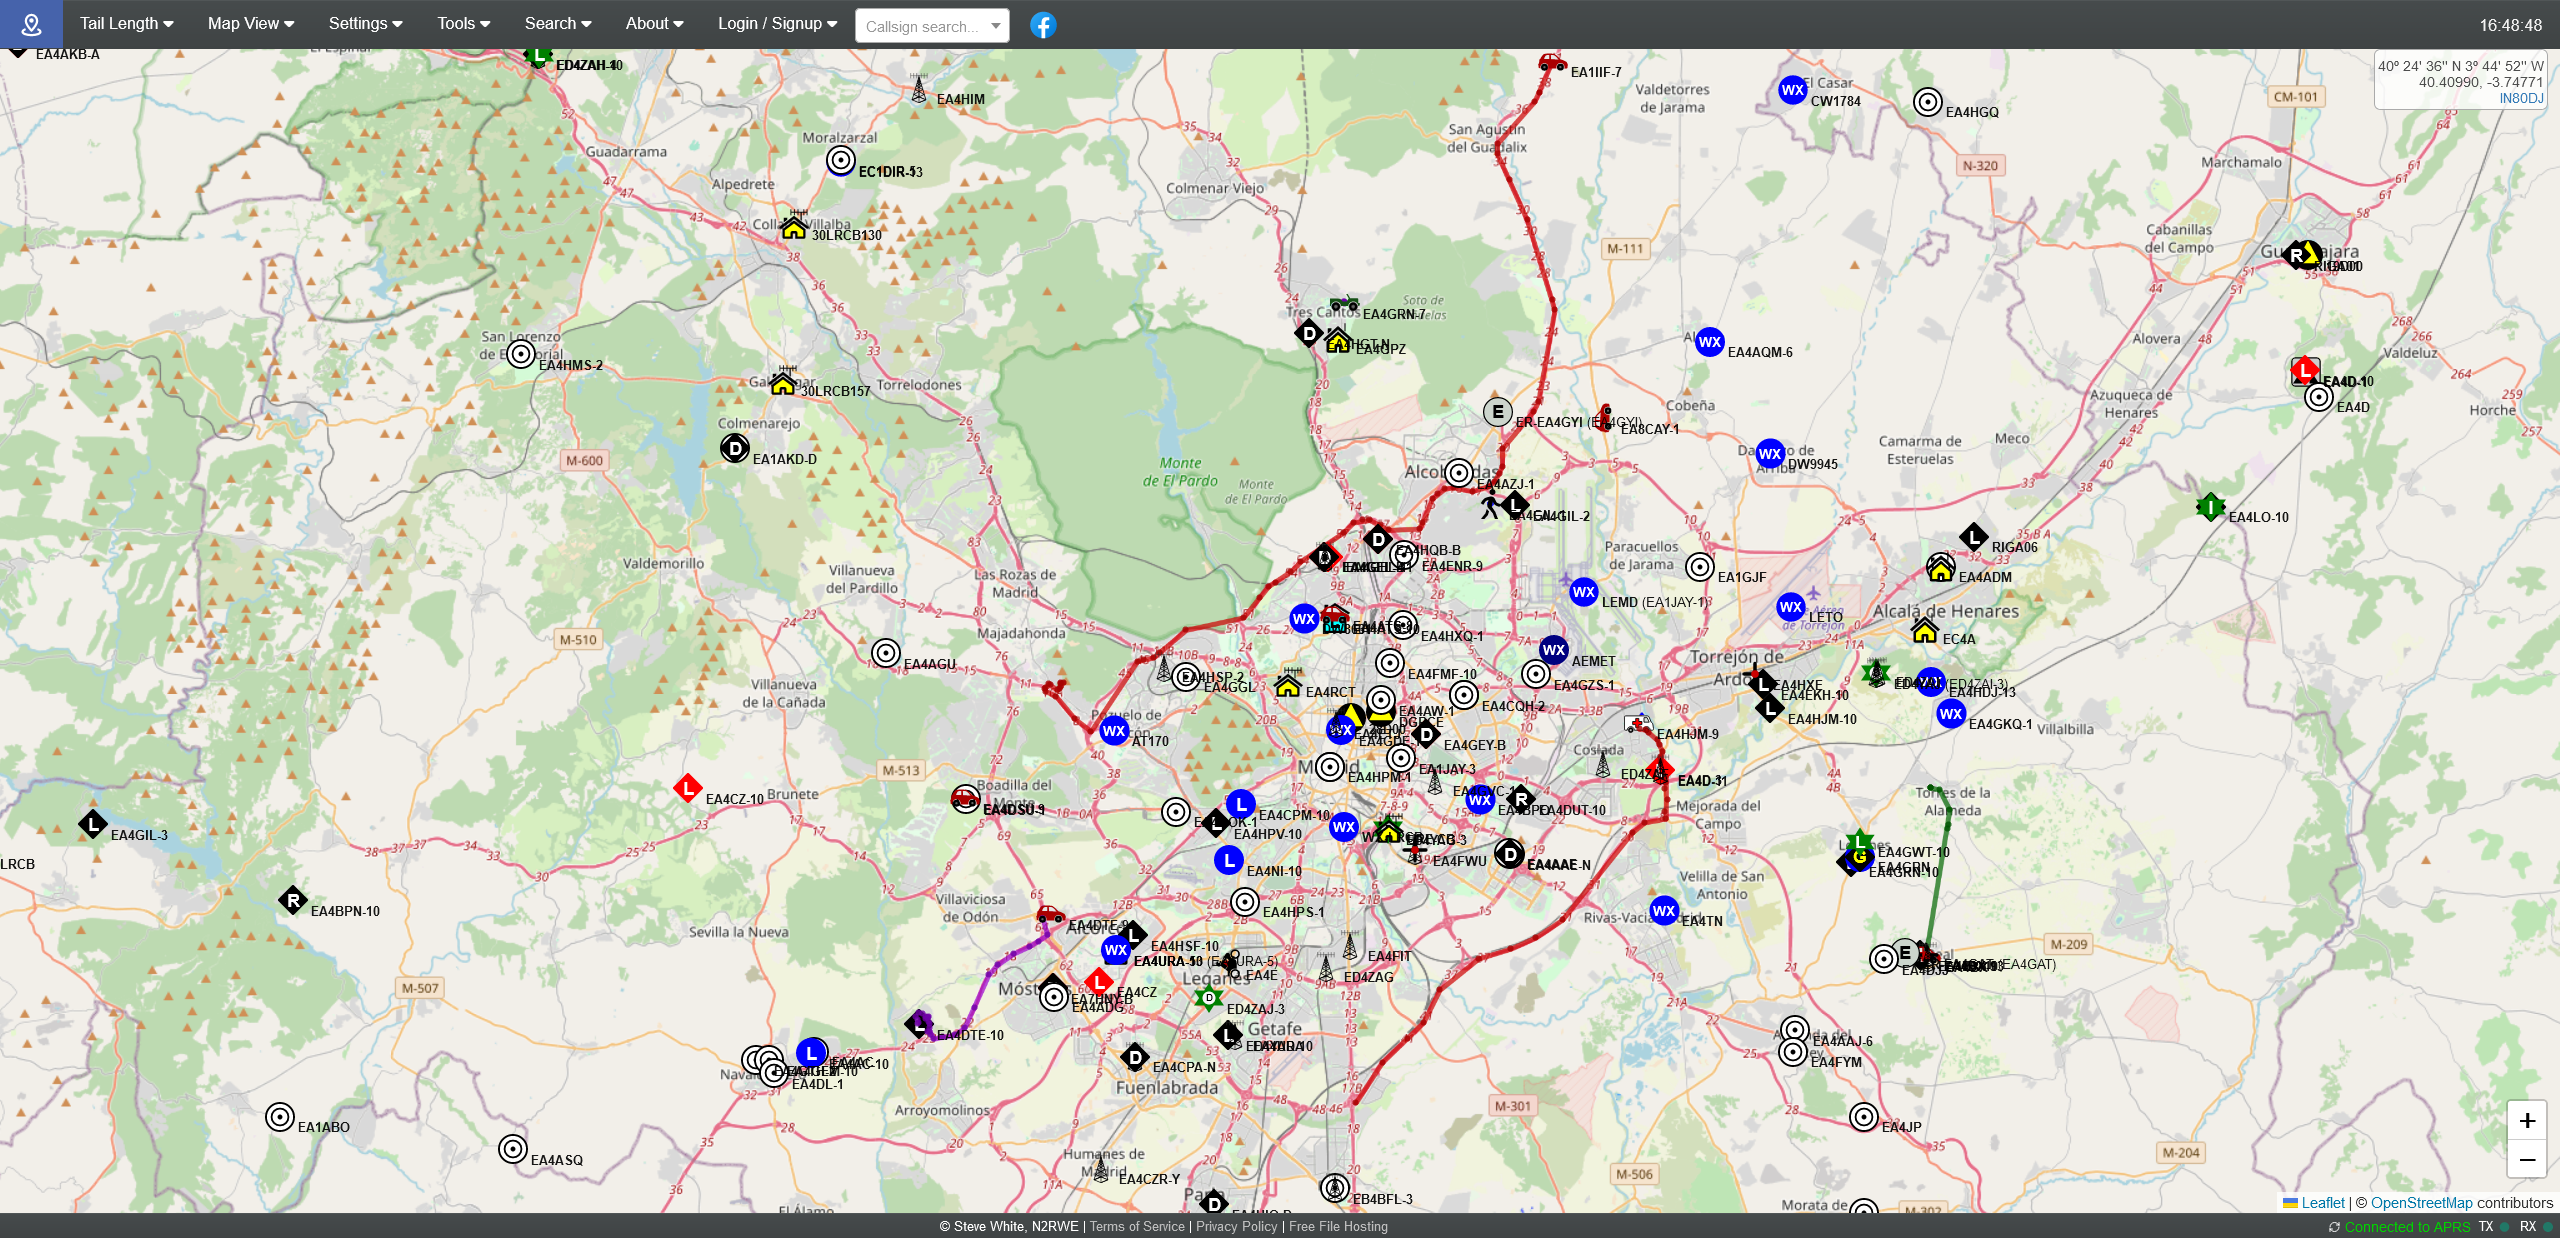
\includegraphics[width=0.7\textwidth]{./Chapter_2/aprs-to.png}
    \caption{Interfaz de aprs.to}
    \label{fig:aprs-to}
\end{figure}

\subsection{Comparación}

En resumen, aprs.fi, la web de visualización de APRS por excelencia, ofrece una gran base de datos y una gran cantidad de información histórica de datos APRS, pero su interfaz puede resultar algo desactualizada y carece de capacidades avanzadas de filtrado. Por otro lado, aprs.to presenta una interfaz más moderna y permite realizar búsquedas básicas y aplicar filtros, aunque también requiere crear una cuenta para acceder a ciertas funciones. Ambas plataformas tienen puntos fuertes y débiles y por esa razón lo mejor es usarlas en conjunto.

	\chapter{Idea}
	\blindtext
	\titleformat{\chapter}[display]
{\normalfont\huge\bfseries}{Capítulo \thechapter}{0.5em}{\huge}
\titlespacing*{\chapter}{0pt}{-1.25cm}{25pt}
\chapter{Arquitectura e Implementación}

En este capítulo se describirá la arquitectura de la aplicación, así como las tecnologías utilizadas para su implementación.

\section{Arquitectura}

Se pueden categorizar los tres módulos (\textbf{Adquisición de datos}, \textbf{Procesamiento y análisis}, \textbf{Visualización y Presentación}) de la aplicación mencionados en el capítulo anterior en dos categorías principales:

\begin{itemize}
	\item \textbf{Adquisición de paquetes APRS:} En este módulo se encuentran los componentes encargados de la adquisición de paquetes APRS. Estos componentes se encargan de recibir los paquetes APRS, procesarlos y almacenarlos en la base de datos de la aplicación.

	\item \textbf{Aplicación web APRSINT:} En este módulo se encuentran los componentes encargados del análisis, la interpretación y la visualización, de los datos almacenados en la base de datos de la aplicación. Estos componentes se encargan de presentar la información de manera rápida y cómoda para el usuario.
\end{itemize}

\section{Tecnologías utilizadas (Marco Teórico)}

Como se ha mencionado anteriormente, uno de los objetivos de APRSINT es el de ser una solución accesible y fácil de usar. Para lograr este objetivo, se han seleccionado tecnologías ampliamente utilizadas y bien documentadas. A continuación se describen las tecnologías utilizadas en cada uno de los módulos de la aplicación.
\subsection{Raspberry Pi}

La Raspberry Pi es un \textit{Single board computer (SBC)} u ordenador de placa única desarrollada por la Fundación Raspberry Pi. Las Raspberry pi son muy populares en el mundo de la informática y la electrónica por su bajo precio, reducido tamaño y su versatilidad.

\begin{itemize}
	\item \textbf{Bajo precio:} La Raspberry es una opción económica para implementar desde prototipos hasta aplicaciones simples, lo que la hace muy accesible para una amplia gama de usuarios.
	\item \textbf{Bajo Consumo Energético:} Su diseño de bajo consumo energético la hace ideal para aplicaciones que requieren funcionamiento continuo.
	\item \textbf{Versatilidad:} La Raspberry Pi 4 es altamente versátil y puede adaptarse a una variedad de casos de uso, desde servidores ligeros hasta placas de desarrollo para robótica y automatización.
\end{itemize}
Se ha seleccionado la Raspberry Pi 4B\footnote{Cuando se comenzó el proyecto todavía no se había lanzado la versión 5.} de 8GB de memoria RAM como plataforma de hardware para la implementación de la solución, debido a sus características y capacidades.

\subsection{Disco duro ssd}
Los discos duros de estado sólido (SSD) son una alternativa a los discos duros tradicionales (HDD) que ofrecen una mayor velocidad de lectura y escritura, menor consumo energético y mayor durabilidad. Se ha seleccionado un disco duro SSD de 250GB que se haya conectado a la Raspberry-pi para almacenar el gran volumen de datos que consume y genera la aplicación a su velocidad y fiabilidad.

\subsection{Python}
Python es un lenguaje de programación interpretado, de alto nivel y de propósito general. Es ampliamente utilizado en el desarrollo de aplicaciones web, científicas y de análisis de datos debido a su simplicidad, flexibilidad y facilidad de uso. Se ha seleccionado Python como lenguaje de programación principal para la implementación de la solución debido a la gran versatilidad que ofrece y sobre todo por la existencia de extensas librerías de visualización y manejo de grandes volúmenes de datos.

\subsection{Dash}
Dash es un framework de Python creado por Plotly para la creación de aplicaciones web interactivas y visualizaciones de datos. Dash permite crear aplicaciones web interactivas y visualizaciones de datos atractivas utilizando Python como lenguaje de programación. Dash esta construido encima de React Se ha seleccionado Dash como framework para la implementación de la interfaz web de la aplicación debido a su facilidad de uso y a la gran cantidad de funcionalidades que ofrece. Dash está escrito encima de Plotly.js, React y Flask lo que permite una gran capacidad de personalización.

\begin{itemize}
	\item \textbf{Interactividad:} Dash permite crear aplicaciones web altamente interactivas, lo que facilita la exploración de datos y la toma de decisiones.
	\item \textbf{Flexibilidad:} Su arquitectura modular y su amplia gama de componentes permiten la creación de aplicaciones web personalizadas y adaptadas a las necesidades específicas del usuario.
	\item \textbf{Integración con Plotly:} Al estar desarrollado por Plotly, Dash ofrece una integración perfecta con las capacidades de visualización de datos de Plotly, lo que permite crear gráficos y visualizaciones muy atractivas.
\end{itemize}

Para crear la aplicación web se consideraron algunas alternativas como Django, Streamlit y PowerBI, sin embargo, Dash fue la opción escogida debido a su extensa capacidad de personalización y personalización de la que carecían las demás opciones.

\subsection{Cosmograph JS}

Cosmograph es una librería de JavaScript enfocada en la visualización de grandes grafos y redes complejas en aplicaciones web. Permite representar de manera interactiva relaciones entre entidades, facilitando la comprensión y el análisis de datos estructurados.

\begin{itemize}
	\item \textbf{Visualización de Grafos:} Cosmograph ofrece herramientas avanzadas para la representación visual de grafos como lineas temporales, histogramas y búsquedas de nodos, una mayor comprensión y capacidad de análisis de la información.

	\item \textbf{Rendimiento:} Cosmograph a diferencia de otras librerías más populares como Sigma JS transfiere todos los cálculos de posiciones de los nodos y aristas así como la representación gráfica de este a la GPU. Esto permite la visualización de grafos con miles de nodos y aristas sin afectar el rendimiento de la aplicación.

	\item \textbf{Personalización:} Ofrece opciones de personalización para adaptar la apariencia y el comportamiento de los nodos y aristas según las necesidades específicas del usuario.

\end{itemize}

Después de una gran cantidad de pruebas y tras considerar muchas alternativas como Sigma-JS, CytoScape y networkx, se acabó eligiendo Cosmograph sobre todo por su rendimiento.

\subsection{PostgreSQL}

PostgreSQL es un sistema de gestión de bases de datos relacional de código abierto y potente, conocido por su fiabilidad, robustez y capacidad para manejar grandes volúmenes de datos. Ofrece una amplia gama de características avanzadas que lo hacen adecuado para aplicaciones web y empresariales exigentes.

\begin{itemize}
	\item \textbf{Fiabilidad y Robustez:} PostgreSQL es conocido por su alta fiabilidad y capacidad para manejar grandes cargas de trabajo sin sacrificar el rendimiento.
	\item \textbf{Escalabilidad:} Es altamente escalable y puede manejar grandes volúmenes de datos y transacciones concurrentes sin problemas.
	\item \textbf{Funcionalidades Avanzadas:} Ofrece una amplia gama de funcionalidades avanzadas, como soporte para transacciones ACID, vistas materializadas, procedimientos almacenados y Full Text Search (búsqueda de indizada).
	\item \textbf{Almacenamiento de datos semiestructurados:} PostgreSQL es capaz de almacenar y manipular datos no estructurados como JSON de manera eficiente, lo que lo hace adecuado para aplicaciones que requieren almacenamiento de datos semiestructurados.
	\item \textbf{Rendimiento:} PostgreSQL ofrece un rendimiento sólido, especialmente en entornos de alta concurrencia y cargas de trabajo intensivas.
\end{itemize}

La elección de PostgreSQL como sistema de gestión de bases de datos se debió a su robustez, facilidad de uso y a la gran cantidad de funcionalidades que ofrece.

\subsection{Sqlalchemy}
SQLAlchemy es una biblioteca de Python que facilita la interacción con bases de datos relacionales utilizando un enfoque orientado a objetos. Permite trabajar con diferentes motores de bases de datos, como PostgreSQL, MySQL, SQLite, entre otros, de una manera consistente y eficiente.

\begin{itemize}
	\item \textbf{Abstracción de la Base de Datos:} SQLAlchemy proporciona una capa de abstracción sobre la base de datos, lo que permite a los desarrolladores interactuar con la base de datos utilizando objetos de Python en lugar de consultas SQL directas.
	\item \textbf{Compatibilidad con Múltiples Motores:} Es compatible con una variedad de motores de bases de datos, lo que brinda flexibilidad para trabajar con diferentes sistemas de gestión de bases de datos según las necesidades del proyecto. En este caso se ha utilizado el motor pysycopg2 para la conexión con PostgreSQL.
	\item \textbf{ORM (Mapeo Objeto-Relacional):} Ofrece un ORM potente y flexible que mapea objetos Python a tablas de bases de datos, facilitando el manejo de relaciones entre objetos y la persistencia de datos.
	\item \textbf{Seguridad:} SQLAlchemy proporciona herramientas para prevenir ataques de inyección SQL y otros problemas de seguridad comunes en el manejo de bases de datos.
\end{itemize}

La elección de SQLAlchemy se ha basado en su capacidad para mejorar el proceso de interacción con la base de datos. Permitiendo una estrecha integración entre la base de datos y la aplicación, permitiendo una flexibilidad muy grande a la hora de hacer consultas o inserciones y sobre todo creando una capa de seguridad para evitar ataques.
\subsection{aprslib}
aprslib es una biblioteca de Python que facilita la interacción con el sistema APRS. Permite recibir y decodificar paquetes APRS, así como enviar paquetes APRS a través de la red APRS-IS.
\begin{itemize}
	\item \textbf{Recepción de Paquetes:} aprslib permite recibir paquetes APRS de la red APRS-IS de manera sencilla.
	\item \textbf{Decodificación de Paquetes:} Facilita la decodificación de paquetes APRS, permitiendo extraer información útil como la posición, velocidad y rumbo de los objetos rastreados.
	\item \textbf{Envío de Paquetes:} aprslib permite enviar paquetes APRS a través de la red APRS-IS, lo que facilita la integración con el sistema APRS.
\end{itemize}
Se ha elegido la librería aprslib por su facilidad de uso, su documentación y su capacidad para decodificar los paquetes APRS.

\subsection{AWS}
Amazon Web Services (AWS) es una plataforma de servicios en la nube ofrecida por Amazon. Proporciona servicios de infraestructura informática, almacenamiento, bases de datos, análisis e inteligencia artificial, entre otros.

\begin{itemize}
	\item \textbf{Fiabilidad:} La infraestructura global de AWS está diseñada para ser altamente disponible y resistente a fallos, lo que garantiza la continuidad del servicio y la seguridad de los datos.
	\item \textbf{Variedad de Servicios:} AWS ofrece una amplia gama de servicios, desde almacenamiento y bases de datos hasta aprendizaje automático y análisis de datos, lo que permite a las empresas construir y desplegar una amplia variedad de aplicaciones y soluciones.
	\item \textbf{Flexibilidad:} AWS proporciona opciones flexibles de implementación, incluyendo la capacidad de utilizar infraestructura física, virtual o basada en contenedores, según las necesidades del proyecto.
	\item \textbf{Seguridad:} AWS cuenta con robustas medidas de seguridad para proteger los datos y las aplicaciones, incluyendo controles de acceso, cifrado de datos y protección contra amenazas.
\end{itemize}

La elección de AWS así como los detalles de la implementación en la nube se describirán en la siguiente sección.

\subsection{Supervisord}
Supervisor es un sistema de control de procesos para sistemas operativos tipo Unix, diseñado para iniciar, detener y gestionar procesos de manera sencilla y robusta. Permite supervisar y mantener en funcionamiento aplicaciones y servicios, reiniciándolos automáticamente en caso de fallos o reinicios del sistema.

\begin{itemize}
	\item \textbf{Gestión de Procesos:} Supervisor facilita la gestión de procesos al permitir iniciar, detener, reiniciar y supervisar procesos de manera centralizada.
	\item \textbf{Monitorización:} Supervisor proporciona información detallada sobre el estado de los procesos, incluyendo registros de eventos y estadísticas de rendimiento.
	\item \textbf{Reinicio Automático:} En caso de fallos, Supervisor puede reiniciar automáticamente los procesos afectados, minimizando el tiempo de inactividad y manteniendo la disponibilidad del servicio.
\end{itemize}

Se ha seleccionado Supervidord como gestor de procesos gracias a su facilidad, flexibilidad (permitiendo ejecutar scripts de Python directamente) y robustez.

\subsection{Pandas}
Pandas es la librería de facto de Python para el manejo y análisis de datos estructurados. Está escrita sobre Numpy (escrito en c) por lo que cuenta con muy buen rendimiento. Esta librería permite la lectura y escritura de datos en diferentes formatos, la manipulación de datos, la limpieza de datos y la creación de gráficos.
\subsection{Apache Airflow}
Apache Airflow es una plataforma de orquestación de tareas y flujos de trabajo. Es similar a Cron de Unix, pero permite una mayor personalización y control de las tareas que ejecuta. Las tareas se definen en archivos separados facilitando la compartimentalización y ofreciendo una mayor robustez y escalabilidad.
\begin{itemize}
	\item \textbf{Orquestación de Flujos de Trabajo:} Airflow facilita la orquestación de flujos de trabajo complejos al permitir definir tareas y sus dependencias como DAG's, lo que proporciona una visión clara de la lógica de ejecución.
	\item \textbf{Escalabilidad:} Airflow es altamente escalable y puede manejar flujos de trabajo de cualquier tamaño, desde tareas simples hasta flujos de trabajo altamente complejos.
	\item \textbf{Monitoreo y Alertas:} Proporciona una interfaz de usuario web para monitorear el estado de los flujos de trabajo, así como capacidades de alerta para detectar y responder a fallos o retrasos en la ejecución de tareas.
	\item \textbf{Extensibilidad:} Airflow es altamente extensible y permite integrar fácilmente con otros sistemas y herramientas, lo que permite construir flujos de trabajo personalizados que se adapten a las necesidades específicas del proyecto.
\end{itemize}

\section{Adquisición de datos}
En esta sección se describirá con detalle el módulo de adquisición de datos de la aplicación, incluyendo la arquitectura, los componentes y las tecnologías utilizadas.
\subsection{RTL-SDR}
En la primera fase del proyecto se compró un dongle RTL-SDR con el fin de recibir los paquetes APRS y procesarlos a partir de ello. Estos dongles son relativamente baratos oscilando entre los 30 y 100 euros, se conectan mediante usb al ordenador y tienen en la parte superior un conector SMA para conectar una antena. La peculiaridad de estos dispositivos reside en que son controlables mediante software y se pueden sintonizar en un rango de frecuencias muy amplio (24MHz a 1.7GHz).

Para hacer uso de estos dispositivos se ha de usar software como GQRX, CubicSDR o SDRSharp. Es posible también usar rtl-sdr en la terminal creando posteriormente un micrófono virtual para que el software de análisis pueda decodificar los paquetes.

Tras multitud de pruebas fallidas con distintos software de visualización y análisis y software de audio como Direwolf, se decidió no continuar por ese camino y probar otras alternativas como la que finalmente se ha implementado el \textbf{APRS-IS}

\subsection{APRS-IS}
APRS-IS es un sistema que permite la transmisión de mensajes APRS por la red de Internet. La ventaja que ofrece este sistema frente al de recopilar información mediante una antena es que APRS-IS, permite obtener un flujo de datos mucho mayor, ya que hay una gran cantidad de antenas y otra ventaja con la que cuenta es que no está restringido al área que puede recibir la pequeña antena rtl-sdr sino a todo el mundo.

\subsubsection{Infraestructura de la red APRS-IS}
Componentes principales:
\begin{itemize}
	\item \textbf{Trackers o TNC:} Son los emisores de los paquetes APRS, suelen corresponder a estaciones fijas o móviles que envían por radio los paquetes con información de posición, velocidad, rumbo, etc.
	\item \textbf{Digipeaters:} Son estaciones que reciben los paquetes APRS y los retransmiten, permitiendo que los paquetes lleguen a una mayor distancia. Son análogos a los repetidores de internet.
	\item \textbf{I-Gates:} Son estaciones que reciben los paquetes APRS por radio y los envían a la red APRS-IS, permitiendo que los paquetes sean accesibles a través de internet.
	\item \textbf{Servidores APRS-IS:} Son servidores que reciben los paquetes APRS de los I-Gates y los almacenan en una base de datos, permitiendo que los clientes accedan a los paquetes a través de internet. Los servidores APRS-IS suelen estar distribuidos geográficamente para mejorar la disponibilidad y la redundancia.
	\item \textbf{Clientes APRS-IS:} Pueden ser otros servidores, aplicaciones web o aplicaciones móviles que acceden a los servidores APRS-IS para obtener los paquetes APRS y mostrarlos a los usuarios.
\end{itemize}
Se muestra el flujo de datos de la red APRS-IS en la \Cref{fig:aprs-infra}.
\begin{figure}[!h]
	\centering
	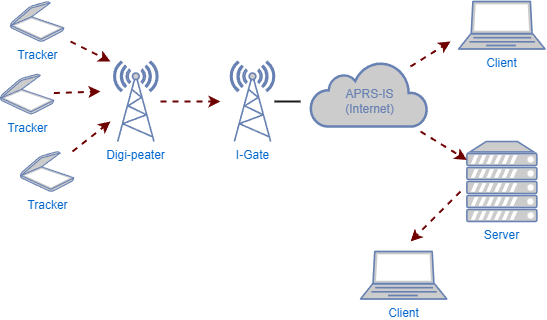
\includegraphics[width=0.85\textwidth]{./Chapter_4/aprs_infra.png}
	\caption{Infraestructura de la red APRS - APRS-IS.}
	\label{fig:aprs-infra}
\end{figure}

Se ha seleccionado APRS-IS como fuente de datos para la aplicación debido a su facilidad de uso, su disponibilidad y la gran cantidad de información que ofrece.

\subsection{Recepción de paquetes APRS}
Para la recepción de paquetes APRS se ha utilizado la librería aprslib de Python. Esta librería permite conectarse a un servidor APRS-IS y recibir los paquetes APRS en tiempo real. Se ha creado un sistema que utilizando esta librería se conecta a un servidor APRS-IS, recibe los paquetes APRS y los guarda en un buffer en memoria. Cuando el buffer se llena con aproximadamente 10.000 mensajes en aproximadamente 15 segundos, se procede a escribir el buffer en un fichero comprimido en el disco duro SSD.
Una cosa curiosa es que los mensajes APRS no se decodifican en este punto, de hecho se guardan sin ningún tipo de procesamiento en ficheros binarios comprimidos en formato gzip para no ocupar mucho espacio en disco. Esto se hace así para evitar la sobrecarga de procesamiento en la Raspberry pi y para poder procesar los mensajes en un servidor más potente en la nube.

Es importante mencionar que el sistema de recepción de paquetes APRS se ejecuta en segundo plano en modo demonio utilizando el gestor de procesos Supervisord, lo que garantiza que el sistema se mantenga en funcionamiento incluso en caso de fallos o reinicios del sistema.

\subsection{Procesado de paquetes APRS}
\subsubsection{Subida de ficheros a AWS S3}
Una vez los ficheros se han guardado en el disco duro SSD, se procede a subirlos a un Bucket S3 en AWS. Para ello se ha utilizado la librería boto3 de Python, que permite interactuar con los servicios de AWS desde Python. Se ha creado un script que se ejecuta una vez al día mediante la orquestación de Apache Airflow y que sube los ficheros comprimidos al bucket S3. Una vez subidos los ficheros, se eliminan del disco duro SSD para liberar espacio. Cuando un fichero se sube sube a S3 se desencadena un evento
\subsubsection{Procesado de paquetes APRS en AWS lambda}
Una vez los ficheros se han subido a S3, se desencadena un evento que ejecuta una función lambda en AWS. Esta función lambda se encarga de descomprimir el fichero, procesar los mensajes APRS y convertirlos en formato JSON.

Por defecto lambda no puede hacer uso de librerías de terceros por lo que se ha tenido que encapsular la librería aprslib en un fichero .zip, subirlo a lambda y establecerlo como una capa de lambda para poder hacer uso de ella.
Para la descompresión de los ficheros se ha utilizado la librería gzip de Python, que permite leer y escribir ficheros comprimidos en formato gzip.
Para el procesado de los mensajes APRS se ha utilizado la librería aprslib de Python como ya hemos mencionado, que permite decodificar los mensajes APRS y extraer información útil como la posición, velocidad y rumbo de los objetos rastreados en formato clave-valor.
Esta función lambda se ejecuta de manera asíncrona y paralela, lo que permite procesar grandes volúmenes de mensajes APRS de manera eficiente y escalable. Una vez procesados los mensajes APRS, se eliminan los ficheros comprimidos del S3 de entrada (aprsinput) para liberar espacio y evitar duplicados.
Finalmente los mensajes procesados se guardan en un Bucket S3 de salida (aprsoutput) en formato JSON para su posterior descarga. La descarga de los ficheros JSON ocurre una vez al día mediante la orquestación de Apache Airflow y la librería boto3. Estos ficheros (uno por fichero de entrada) se descargan a otra carpeta temporal en la Raspberry pi.


\subsection{Almacenamiento de paquetes APRS en la base de datos}
Una vez los ficheros JSON ya procesados se han descargado al directorio temporal en la Raspberry pi, se procede a almacenarlos en la base de datos PostgreSQL. Para ello se ha utilizado la librería SQLAlchemy de Python, que permite interactuar con bases de datos relacionales de manera sencilla y eficiente. Se ha creado un script que se ejecuta una vez al día mediante la orquestación de Apache Airflow y que lee los ficheros JSON, procesa los mensajes APRS y los almacena en la base de datos.
Este paso esconde un gran problema que hubo de ser solucionado. El script en un principio seguía los siguientes pasos.

\begin{enumerate}
	\item \textbf{Lectura de ficheros JSON:} El script lee los ficheros JSON de la carpeta local /tmp descargados del bucket S3.
	\item \textbf{Extracción de la estación:} El script extrae la estación origen y destino de cada mensaje y en caso de no existir en la base de datos las crea.
	\item \textbf{Extracción de las posiciones:} Se extraen las posiciones (si las hay) de cada mensaje y el timestamp si lo hay y se almacenan en la base de datos.
	\item \textbf{Identificación del país:} Mediante la librería geopy y ficheros de formas de países se identifica el país de la estación.
	\item \textbf{Extracción de los mensajes:} Se extraen los mensajes de cada línea del JSON y se almacenan en la base de datos.
\end{enumerate}

Este enfoque resultó tener varios problemas. El primero y más importante era el de rendimiento, ya que cada archivo JSON contenía alrededor de 10000 mensajes y en la creación de los objetos, inserciones en la BD y detección del país se tardaba alrededor de 40 segundos por fichero JSON. Esto aunque no parezca demasiado tiempo, si se tiene en cuenta que la cantidad de mensajes APRS que se reciben en 40 segundos es alrededor de 45000 mensajes, se puede ver que el sistema no era escalable.

\subsubsection{\underline{Optimizaciones}}
Para solucionar este problema se realizaron las siguientes optimizaciones:
\begin{itemize}
	\item \textbf{Uso de sets:} Se ha cambiado el uso de consultas a la BD por sets en la creación de las estaciones para acelerar la comprobación la existencia de una estación en la base de datos.
	\item \textbf{Batch Insert:} Se ha modificado la interfaz con Sqlalchemy para permitir inserciones en lotes de 250 mensajes.
	\item \textbf{Detección de países con geopandas:} Se ha cambiado la librería geopy por geopandas que permite la detección de países de manera mucho más rápida utilizando paralelización.
\end{itemize}
Estas optimizaciones han permitido que el tiempo de procesado de un fichero JSON haya pasado de 40 segundos a unos 2 segundos, lo que ha permitido que el sistema sea escalable y pueda procesar grandes volúmenes de mensajes APRS de manera eficiente.

\subsection{Base de datos}
Como se ha mencionado previamente, se ha elegido PostgreSQL como sistema de gestión de bases de datos para la aplicación. Esta elección se ha basado en la robustez, la fiabilidad y la capacidad de manejar grandes volúmenes de datos que ofrece PostgreSQL incluso en sistemas con recursos reducidos. La base de datos se ha diseñado siguiendo un modelo relacional \Cref{fig:db-model} que permite almacenar y relacionar la información de los mensajes APRS de manera eficiente, el modelo cuenta con las siguientes tablas.

\begin{itemize}
	\item \textbf{stations:} Almacena la información de las estaciones APRS, incluyendo el identificador (CALLSIGN), el ssid y su símbolo.
	\item \textbf{station\textunderscore locations:} Almacena la información de las posiciones \footnote[1]{Esta tabla tiene un campo id en la clave primaria por si una estación ha emitido un mensaje sin timestamp} de las estaciones APRS, incluyendo el país, la latitud, la longitud y la fecha y hora en la que se han recibido.
	\item \textbf{messages:} Almacena la información de los mensajes APRS, incluyendo el contenido del mensaje, el tipo de mensaje y el timestamp.
	\item \textbf{qrz\textunderscore profiles:} Sirve como una caché que almacena la información de los perfiles de los usuarios de QRZ, incluyendo el identificador (CALLSIGN), el nombre, la dirección, la ciudad, el estado, el código postal, el país, la latitud, la longitud y la fecha de nacimiento entre muchos otros.
\end{itemize}

\begin{figure}[!h]
	\centering
	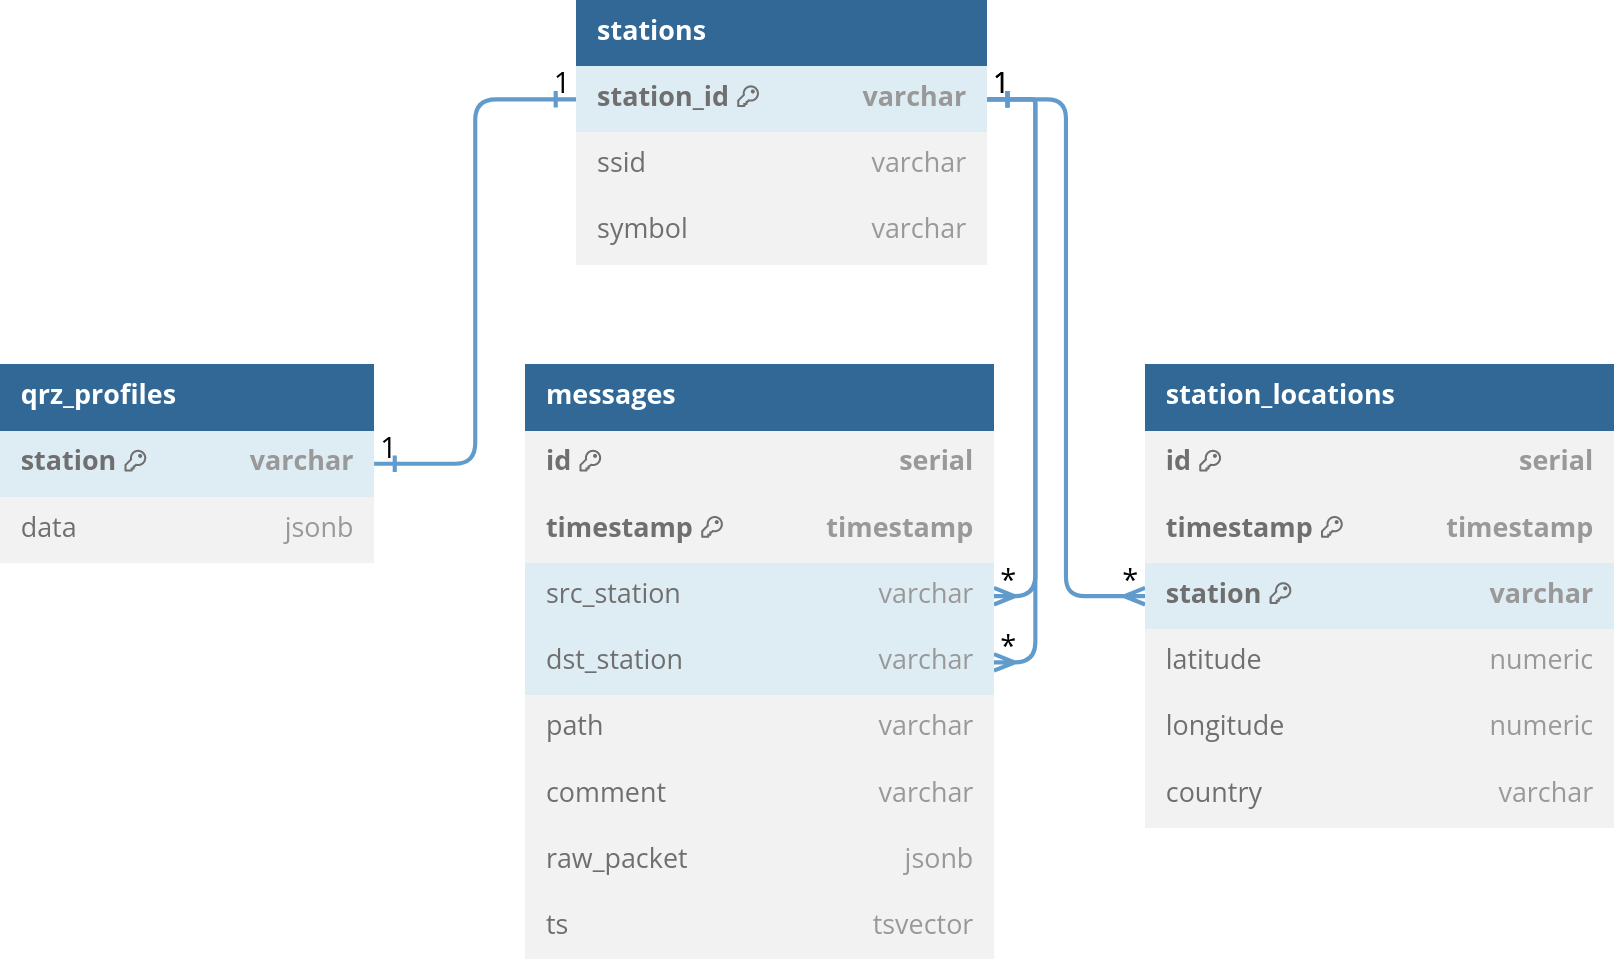
\includegraphics[width=0.85\textwidth]{./Chapter_4/db_diagram.png}
	\caption{Estructura de la base de datos.}
	\label{fig:db-model}
\end{figure}

\section{Visualización y Presentación de datos}

En esta sección se describirá con detalle el módulo de visualización y presentación de datos de la aplicación, incluyendo la arquitectura, los componentes y las tecnologías utilizadas.

\subsection{Dash}
Dash es un framework de Python creado por Plotly para la creación de aplicaciones web interactivas y visualizaciones de datos. Dash permite crear aplicaciones web interactivas y visualizaciones de datos atractivas utilizando Python como lenguaje de programación. Dash está escrito encima de Plotly.js, React y Flask lo que permite una gran capacidad de personalización.
Dash ofrece una versión de pago llamada Dash Enterprise que ofrece una gran cantidad de funcionalidades para elaborar aplicaciones web de manera más rápida y sencilla. Sin embargo, para este proyecto se ha utilizado la versión gratuita de Dash, con algunas librerías adicionales entre las que se encuentran:
\begin{itemize}
	\item \textbf{Dash Core Components:} Ofrece una amplia gama de componentes interactivos como gráficos, tablas, sliders, dropdowns, entre otros, que permiten a los usuarios interactuar con los datos de manera intuitiva.
	\item \textbf{Dash HTML Components:} Ofrece una amplia gama de componentes HTML como divs, spans, inputs, entre otros, que permiten personalizar la apariencia y el diseño de la aplicación web.
	\item \textbf{Dash Mantine Components:} Ofrece una amplia gama de componentes de Mantine como navbars, tarjetas, modales, entre otros, que permiten crear aplicaciones web atractivas y responsivas.
	\item \textbf{Dash Express:} Ofrece componentes extra como un panel de filtrado y una barra de navegación. \footnote{Esta librería se ha modificado para adaptarla a las necesidades del proyecto.}
	\item \textbf{Plotly Express:} Es el principal competidor de matplotlib en el mundo de la visualización de datos en Python. Ofrece una gran cantidad de gráficos y visualizaciones de datos interactivos.
\end{itemize}

\subsection{Diseño}
El diseño de la aplicación web se ha basado en la simplicidad, la usabilidad y la accesibilidad. El primer diseño del proyecto se realizó en la aplicación de prototipado Figma como se muestra en la \Cref{fig:figma}.

\begin{figure}[h]
	\centering
	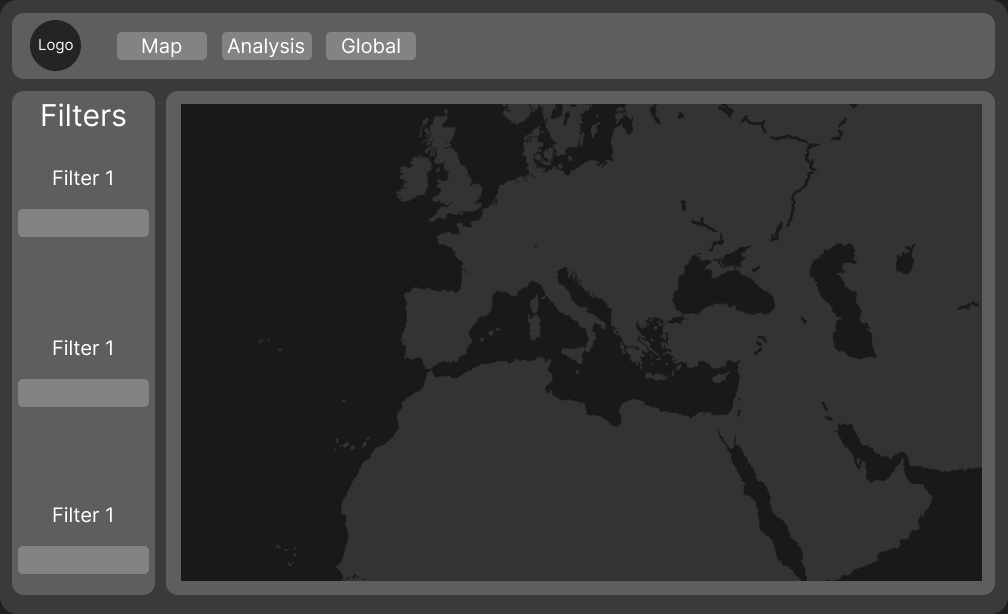
\includegraphics[width=0.6\textwidth]{./Chapter_4/first_draft.png}
	\caption{Primer diseño de la aplicación web en Figma.}
	\label{fig:figma}
\end{figure}

Este diseño se ha ido modificando y adaptando a lo largo del desarrollo del proyecto para mejorar la usabilidad y la experiencia del usuario. Este diseño muestra la pantalla principal de la aplicación, que incluye un mapa con las estaciones APRS, y un panel de control con filtros y opciones de visualización.

\subsection{Home - Primera pantalla}
En esta sección se describirá la primera pantalla de la aplicación web, que muestra un mapa con las estaciones APRS y un panel de control con filtros y opciones de visualización. 
\subsubsection{Obtención de datos}

Siguiendo la estrategia de otros sistemas de dashboarding como PowerBI o Tableau y con el objetivo de mejorar la eficiencia y la escalabilidad del sistema, se ha optado por eliminar en lo posible las consultas a la base de datos en tiempo real. Para ello se ha creado un sistema de caché que almacena los datos a representar en esta pantalla en un archivo de rápida lectura que es actualizado diariamente mediante Apache Airflow. Este sistema de caché permite reducir la carga en la base de datos y mejorar el rendimiento de la aplicación web. 

El sistema de caché se ha implementado utilizando la librería Pandas de Python, usando un fichero .feather para almacenar los datos en formato binario y comprimido y reducir dramáticamente\footnote{Los ficheros de tipo .feather son hasta 100 veces más rápidos que los ficheros .csv} el tiempo de carga de la página.

\subsubsection{Mapa de estaciones APRS}

El mapa de estaciones APRS muestra la posición de cada una de las estaciones APRS, representadas por un marcador en el mapa. Es un mapa interactivo que permite hacer zoom, desplazarse y al posicionar el cursor encima de una estación aparecerá un recuadro ofreciendo información adicional.

Esta página hace uso de la librería Plotly para renderizar el mapa y del servicio web de mapas Mapbox para obtener los mapas y estilos de mapa.

\subsubsection{Filtros}
El panel de control de la aplicación web incluye una serie de filtros y opciones de visualización que permiten al usuario personalizar la información mostrada en el mapa. La ventaja de estos filtros es que son aditivos y se pueden combinar para obtener con exactitud la información requerida. Los filtros disponibles son:
\begin{itemize}
	\item \textbf{Filtro por Rango de Fechas:} Permite filtrar las estaciones APRS por rango de fechas, mostrando solo las estaciones de las que se ha recibido algún mensaje en el rango de fechas seleccionado.
	\item \textbf{Filtro por País:} Permite filtrar las estaciones APRS por país, mostrando solo las estaciones que se encuentran en el país seleccionado.
	\item \textbf{Filtro por contenido del mensaje:} Este es quizás el filtro más interesante, ya que permite filtrar las estaciones por el contenido del mensaje, este filtro será explicado más adelante.
	\item \textbf{Filtro por Tipo de Estación:} Permite filtrar las estaciones APRS por tipo, mostrando solo las estaciones que corresponden al tipo seleccionado.
	\item \textbf{Filtro por ssid:} Permite filtrar las estaciones por ssid.
\end{itemize}

\subsubsection{Búsqueda difusa en contenido de mensajes}
Este filtro es personalmente el más interesante de todos los filtros disponibles. El objetivo es permitir al usuario buscar mensajes emitidos por las estaciones que contengan una palabra o frase especifica. Para ello se han probado varias alternativas como el uso de expresiones regulares o una implementación en Python puro. El problema de estas opciones es que son muy lentas para el enorme volumen de datos con el que se cuenta y al ser dinámico no era factible realizar esa búsqueda en tiempo real.
Finalmente se ha optado por el uso de Postgresql FTS (Full Text Search). Postgres FTS es un sistema de búsqueda de texto completo que permite realizar búsquedas de texto en grandes volúmenes de datos de manera eficiente. Las ventajas que ofrece este sistema son:

\begin{itemize}
	\item \textbf{Rendimiento:} Todo el proceso de búsqueda se realiza en la base de datos, lo que permite realizar búsquedas de texto sin transferir todos los mensajes al servidor para su búsqueda.
	\item \textbf{Búsqueda difusa:} Permite realizar búsquedas de texto difuso, lo que significa que se pueden buscar palabras o frases que contengan errores tipográficos o que no coincidan exactamente con el texto buscado.
	\item \textbf{Indexación:} Postgresql FTS indexa automáticamente los mensajes de texto, lo que permite realizar búsquedas de texto de manera eficiente incluso en grandes volúmenes de datos.
\end{itemize}
Se ha creado un índice de texto completo en la columna de mensajes de la tabla de mensajes y se ha utilizado la función to\textunderscore tsvector para convertir los mensajes en un vector de texto completo. Posteriormente se ha utilizado la función plainto\textunderscore tsquery para convertir la palabra o frase de búsqueda en una consulta de texto completo y finalmente se ha utilizado la función ts\textunderscore query para realizar la búsqueda de texto completo en la columna de mensajes. Este filtro permite al usuario buscar mensajes emitidos por las estaciones que contengan una palabra o frase específica, lo que facilita la identificación y el análisis de los mensajes relevantes.
Cuando un usuario realiza una búsqueda de texto completo, se muestra un modal con la lista de todos los mensajes que contienen la palabra o frase de búsqueda, ordenados por relevancia haciendo uso de la función ts\textunderscore rank. Otra funcionalidad interesante es que la palabra o palabras buscadas se resaltan en el mensaje para facilitar su identificación como se muestra en la \Cref{fig:postgres-fts}.

\begin{figure}[h]
	\centering
	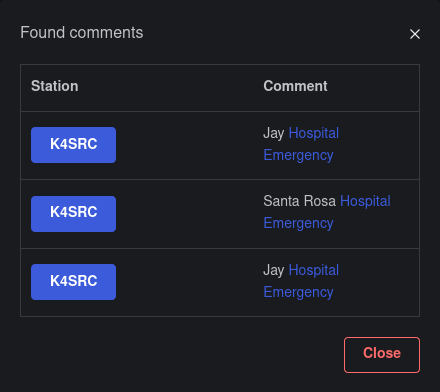
\includegraphics[width=0.5\textwidth]{./Chapter_4/fts_output.png}
	\caption{Resultados de la búsqueda de <<emergency hospital>>.}
	\label{fig:postgres-fts}
\end{figure}

En el modal se muestra una tabla de dos columnas, la columna izquierda contiene un boton con el nombre de la estación y la columna derecha el contenido del mensaje.

\subsection{Station - Segunda pantalla}
Esta es la página que hace única a APRSINT. En esta página se muestra la información detallada de una estación APRS en concreto. Se puede llegar a esta pantalla desde la página principal haciendo clic en un marcador de una estación en el mapa, haciendo clic en una estación en la búsqueda en los mensajes o haciendo clic en un nodo del grafo de la página 3. La pantalla station está dividida en tres secciones.

\subsubsection{Información de QRZ}
QRZ es una base de datos de radioaficionados que contiene información detallada sobre los radioaficionados de todo el mundo. Para acceder a la información disponible en la web \url{qrz.com} es necesario tener una cuenta y estar registrado. QRZ cuenta con un servicio de API que permite acceder a la información de los radioaficionados de manera programática. Para mantener APRSINT fiel a los principios del OSINT (fuentes abiertas) se ha optado por no utilizar la API e intentar otra opción.

Utilizando una cuenta normal gratuita en QRZ, se permiten realizar hasta 25 visualizaciones de perfiles diarias en su sitio web. Con el objetivo de aumentar la cantidad de visualizaciones disponibles, se ha optado por implementar web scraping mediante un sistema propio de rotación de cuentas gratuitas y utilizando la librería \textit{BeautifulSoup}. Como parte de esta estrategia, se ha creado una tabla en la base de datos para almacenar en caché las solicitudes, lo que reduce el número de solicitudes a una misma estación si esta ya ha sido consultada previamente.

Este módulo es de los más complejos de la aplicación, pero a su vez de los más útiles, ya que permite al usuario obtener información muy detallada de una estación APRS en concreto y de la persona que está detrás. Algunos de los datos que se pueden obtener son:

\begin{itemize}
	\item Nombre de la persona registrada
	\item Fechas de registro y última actualización en la web
	\item Alias conocidos de la estación
	\item Dirección de la persona registrada (Como link a google maps)
	\item Fecha de nacimiento de la persona registrada
\end{itemize}

\subsubsection{Información de posiciones}
Esta sección se compone de dos partes. En la parte superior se muestra un mapa con todas las posiciones reportadas por la estación, se muestra también la caja delimitadora de todas las posiciones. 

En la parte inferior se muestran estadísticas de las posiciones reportadas por la estación como la frecuencia media de emisión, la primera y última emisión recibida y por cada mensaje emitido por la estación se muestra el número de repeticiones del mensaje y las urls (si existen) encontradas en los mensajes.

\subsubsection{Información de mensajes}
Finalmente encontramos la sección de mensajes. En esta sección se muestra una tabla en la que se muestra la información de los mensajes emitidos por la estación. La tabla se compone de las siguientes columnas:
\begin{itemize}
	\item La fecha de emisión del mensaje.
	\item La latitud y longitud de la estación en el momento de la emisión.
	\item El país en el que se encontraba la estación en el momento de la emisión.
	\item La estación destino del mensaje.
	\item El \textit{path} es decir los digipeaters que han retransmitido el mensaje.
	\item El contenido del mensaje.
\end{itemize} 

La tabla es interactiva y permite al usuario filtrar los mensajes por el intervalo de fechas que pretenda.

\subsection{Graph - Tercera pantalla}
Esta pantalla es la última de la web, en ella se muestra un grafo dirigido en el que los nodos son las estaciones y las aristas dirigidas, mensajes como se muestra en la \Cref{fig:graph}. El grafo es interactivo y permite hacer zoom, desplazarse y al posicionar el cursor encima de un nodo o arista aparecerá un recuadro ofreciendo información adicional. El color y tamaño de los nodos depende de la cantidad de mensajes que ha emitido o recibido la estación y de misma manera el color y tamaño de las aristas depende de la cantidad de mensajes que se han emitido o recibido desde la estación origen y destino.

\begin{figure}[h]
	\centering
	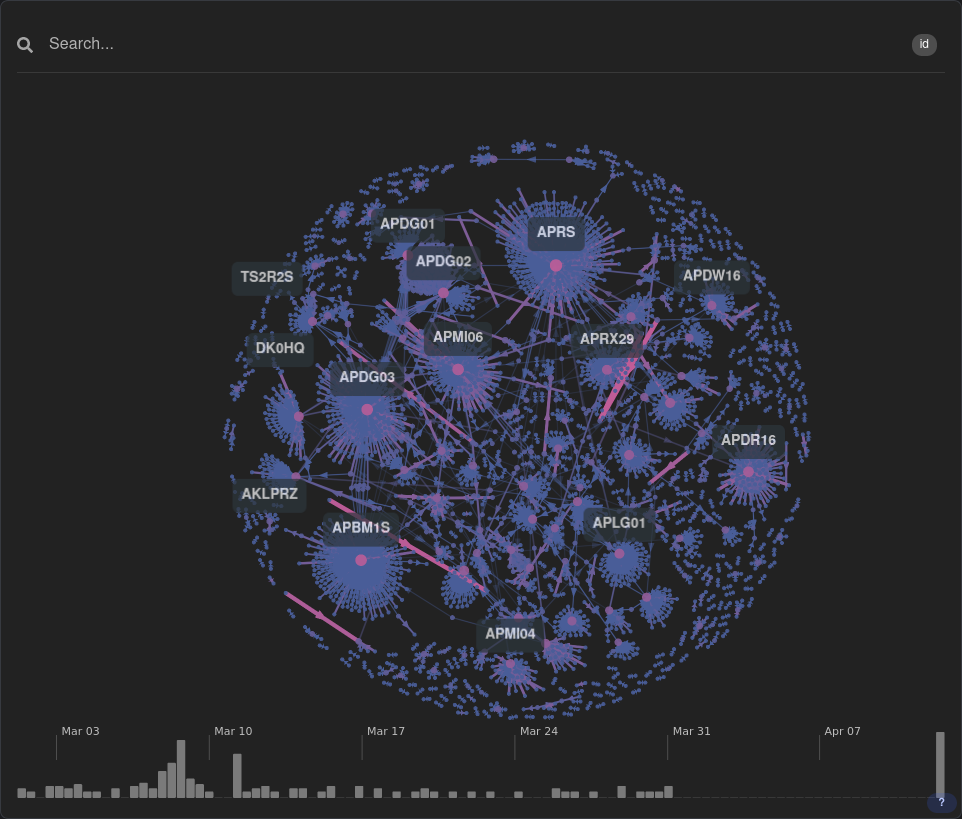
\includegraphics[width=0.7\textwidth]{./Chapter_4/graph.png}
	\caption{Grafo de estaciones APRS.}
	\label{fig:graph}
\end{figure}

Las características que se buscaban en la solución final eran:

\begin{itemize}
	\item \textbf{Interactividad:} Se buscaba un grafo interactivo que permitiera al usuario explorar las relaciones entre las estaciones APRS.
	\item \textbf{Rendimiento:} Quizás la característica más importante, el grafo debía ser capaz de mostrar una gran cantidad de estaciones y conexiones sin afectar al rendimiento de la aplicación.
	\item \textbf{Personalización:} Se buscaba un grafo que permitiera personalizar la apariencia y el comportamiento de los nodos y aristas según las características de cada estación y mensaje.
\end{itemize}
Para alcanzar la solución final que se presenta ahora en la página, se han probado muchas opciones que se han ido descartando por diferentes motivos.
\subsubsection{Alternativas probadas}
En un primer momento se intentó utilizar la librería \textbf{networkx} de Python para la creación del grafo, sin embargo, se descartó debido a su rendimiento y a su falta de interactividad. Posteriormente se intentó utilizar la librería \textbf{Cytoscape} que es la solución por defecto que ofrece Dash, esta ofrece una gran cantidad de funcionalidades para la creación de grafos interactivos, sin embargo, se descartó de nuevo debido a su pobre rendimiento.

Una de las alternativas que también se probó fue la librería \textbf{Sigma JS} que ofrece una gran cantidad de funcionalidades y personalización para la creación de grafos interactivos. Esta librería cuenta con una funcionalidad interesante \textit{forceAtlas2} que permite calcular mediante una simulación de fuerzas la posición de los nodos y aristas en el grafo. Sin embargo, de nuevo se descartó debido a su rendimiento con una gran cantidad de nodos y aristas.

Finalmente se optó por la librería \textbf{Cosmograph JS}. Cosmograph utiliza la librería \textit{cosmos} de cálculo de posiciones mediante la GPU y por tanto puede manejar un gran número de nodos y aristas.

\subsubsection{El grafo}
El problema principal con Cosmograph ha sido la falta de documentación debido a que es bastante nueva y la dificultad de integrarla con Dash. Esta librería está publicada en npm (el repositorio de librerias de JavaScript) y se ha tenido que utilizar bundle.js para convertir el código de JavaScript en un solo fichero que se pueda importar en Dash. Ha sido necesario modificar ligeramente la librería para terminar de integrarla con Dash.

Se han utilizado tres componentes de Cosmograph JS para la creación del grafo, el componente \textit{Cosmograph} que crea el grafo, el componente \textit{CosmographSearch} que permite mediante una barra de búsqueda encontrar una estación y el componente \textit{CosmographTimeline} que permite filtrar el grafo por rango de fechas.

Para mejorar el rendimiento general de la web se ha utilizado la técnica de lazy-loading, que consiste en cargar los componentes del grafo solo cuando el usuario presiona el botón \textit{Load graph}. En el momento que el usuario presiona el botón, se activa un callback de cliente de Dash. El callback primero lee los datos del grafo de un fichero CSV que se actualiza diariamente mediante Apache Airflow. Posteriormente se crean los nodos y las aristas y se inicializa el grafo, la barra de búsqueda y la barra de tiempo. Seguidamente se establecen los parámetros de la simulación de fuerzas y se inicia la simulación. Por último se establecen las propiedades visuales y funcionales de los nodos y aristas.

Cuando el usuario arrastra el cursor sobre un nodo, se muestra un recuadro con el nombre de la estación. Cuando el usuario hace clic en un nodo, se le redirige a la página \textbf{station} de la estación seleccionada.

\section{Orquestación}

En esta sección se describirá con detalle la metodología de orquestación de tareas y flujos de trabajo de la aplicación que se han ido comentando a lo largo del capítulo.

\subsection{Supervisord}
Supervisord es un sistema de control de procesos para sistemas operativos tipo Unix, diseñado para iniciar, detener y gestionar procesos de manera sencilla y robusta.

Se ha utilizado Supervisord como gestor de procesos para ejecutar en modo demonio como se ha mencionado previamente el sistema de recepción de paquetes APRS. Se ha establecido en la configuración de Supervisord que el sistema de recepción de paquetes se ejecute en el arranque del sistema y siempre después de que la interfaz de red esté disponible. En caso de fallo del sistema de recepción, Supervisord reiniciará el sistema y registrará la causa del fallo.

\section{Apache Airflow}
Apache Airflow es una plataforma de orquestación de tareas y flujos de trabajo. Es similar a Cron de Unix, pero permite al usuario una mayor personalización y un mayor control sobre las tareas que controla. La unidad de ejecución en Apache Airflow es el DAG (Directed Acyclic Graph). Las tareas se definen en archivos individuales y al igual que en otros sistemas se pueden definir dependencias entre tareas.

Apache Airflow se ha utilizado para orquestar todas las tareas que permiten que APRSINT funcione correctamente se presenta en la \Cref{tab:airflow-sched} la lista de los DAG's que se ejecutan diariamente.

\begin{table}[htbp]
    \centering
    \begin{tabular}{|c|l|l|}
        \hline
        \textbf{Hora de ejecución} & \textbf{DAG} & \textbf{Descripción} \\
        \hline
        3:00 am & upload\_files & Sube todos los archivos al S3 aprsinput \\
        \hline
        5:00 am & download\_files & Descarga todos los archivos a la carpeta local \\
        \hline
        7:00 am & insert\_database & Inserta todos los mensajes en la BBDD \\
		\hline
        9:00 am & cache\_data & Precalcula en archivos los datos para la web \\
        \hline
    \end{tabular}
    \caption{Esquema de orquestaciÓn con Apache Airflow.}
    \label{tab:airflow-sched}
\end{table}

\section{Alojamiento}
Para alojar tanto la aplicación web como el sistema de recepción de paquetes y la base de datos de APRSINT se ha optado por utilizar una raspberry Pi 4 conectada a un internet residencial. 

Para evitar los problemas que suponen las direcciones dinámicas se ha optado por utilizar el servicio de DNS dinámico de no-ip que permite asignar un nombre de dominio a una dirección IP dinámica. 

\subsection{Servidor Web}
Insertar la solución escogida (Probablemente Nginx)


\subsection{Protección ante ataques}

Para todo el desarrollo de la aplicación se ha utilizado el protocolo ssh.
Se han ampliado las medidas de seguridad de la raspberry pi mediante la creación de un usuario no root. Se ha cambiado el puerto de ssh por defecto y se ha desactivado el acceso por contraseña. Se ha instalado \textbf{fail2ban} para protegerse de ataques de fuerza bruta y se ha instalado un firewall \textbf{UFW} para bloquear el acceso a los puertos no utilizados. 
	\titleformat{\chapter}[display]
{\normalfont\huge\bfseries}{Capítulo \thechapter}{0.5em}{\huge}
\titlespacing*{\chapter}{0pt}{-1.25cm}{25pt}
\chapter{Propuesta de la Idea}

\section{Implementacion y arquitectura}

Aqui hablo de cosas
	\chapter{Conclusiones y trabajo futuro}
	\blindtext


\chapter*{Conclusions and future work}
	Translate the previous chapter
	
	
	
	% %Compact bibliography style
	% \begin{multicols}{2}[\printbibheading]
	% 	\printbibliography[heading=none]
	% 	\addcontentsline{toc}{chapter}{Bibliography}
	% \end{multicols}

\end{document}